\documentclass{ximera}

\graphicspath{
  {./}
  {graphics/}
  {../graphics/}
}

\usepackage{chngcntr}

\let\question\relax
\let\endquestion\relax




\newtheoremstyle{SlantTheorem}{\topsep}{\fill}%%% space between body and thm
%\newtheoremstyle{SlantTheorem}{\topsep}{\topsep}%%% space between body and thm
 {\slshape}                      %%% Thm body font
 {}                              %%% Indent amount (empty = no indent)
 {\bfseries\sffamily}            %%% Thm head font
 {}                              %%% Punctuation after thm head
 {3ex}                           %%% Space after thm head
 {\thmname{#1}\thmnumber{ #2}\thmnote{ \bfseries(#3)}}%%% Thm head spec
\theoremstyle{SlantTheorem}
\newtheorem{question}{Question}
\counterwithin*{question}{section}



\let\instructorNotes\relax
\let\endinstructorNotes\relax
%%% instructorNotes environment
\ifhandout
\newenvironment{instructorNotes}[1][false]%
{%
\def\givenatend{\boolean{#1}}\ifthenelse{\boolean{#1}}{\begin{trivlist}\item}{\setbox0\vbox\bgroup}{}
}
{%
\ifthenelse{\givenatend}{\end{trivlist}}{\egroup}{}
}
\else
\newenvironment{instructorNotes}[1][false]%
{%
  \ifthenelse{\boolean{#1}}{\begin{trivlist}\item[\hskip \labelsep\bfseries {\Large Instructor Notes: \\} \hspace{\textwidth} ]}
{\begin{trivlist}\item[\hskip \labelsep\bfseries {\Large Instructor Notes: \\} \hspace{\textwidth} ]}
{}
}
{\end{trivlist}}
\fi


%% Suggested Timing
\newcommand{\timing}[1]{{\bf Suggested Timing: \hspace{2ex}} #1}

\title{The Graphic Details}
\author{Vic Ferdinand, Betsy McNeal, Jenny Sheldon}
\begin{document}
\begin{abstract}\end{abstract}
\maketitle

\begin{instructorIntro}
Here we begin to inspect graphical representations of functions or expressions rather than algebraic or tabular representations.  You might remind students that we've already studied the algebraic representations if this hasn't been done for some time, and that this is a connection between algebra and geometry.  We don't necessarily have a formula for the graphs in question, only data points.  

You will want to point out that a graph can be dealt with locally, as each point is a special case of the relationship between the variables, as well as globally.  The global point of view tells the story of what happens to one variable as the other variable(s) change.

\timing{This will probably take an entire class period or more.  To shorten the activity you could do only the first two problems. You can divide up the parts amongst the groups, and have them present their solutions to the class, but this will generate a lot less discussion..}

\vskip 3.5in
\end{instructorIntro}

\begin{problem}
For each of the situations below, pick the graph that most reasonably
reflects the situation and the variables involved.

\begin{enumerate}
\item The daily high temperature recorded in Chicago from January to
  December

\[
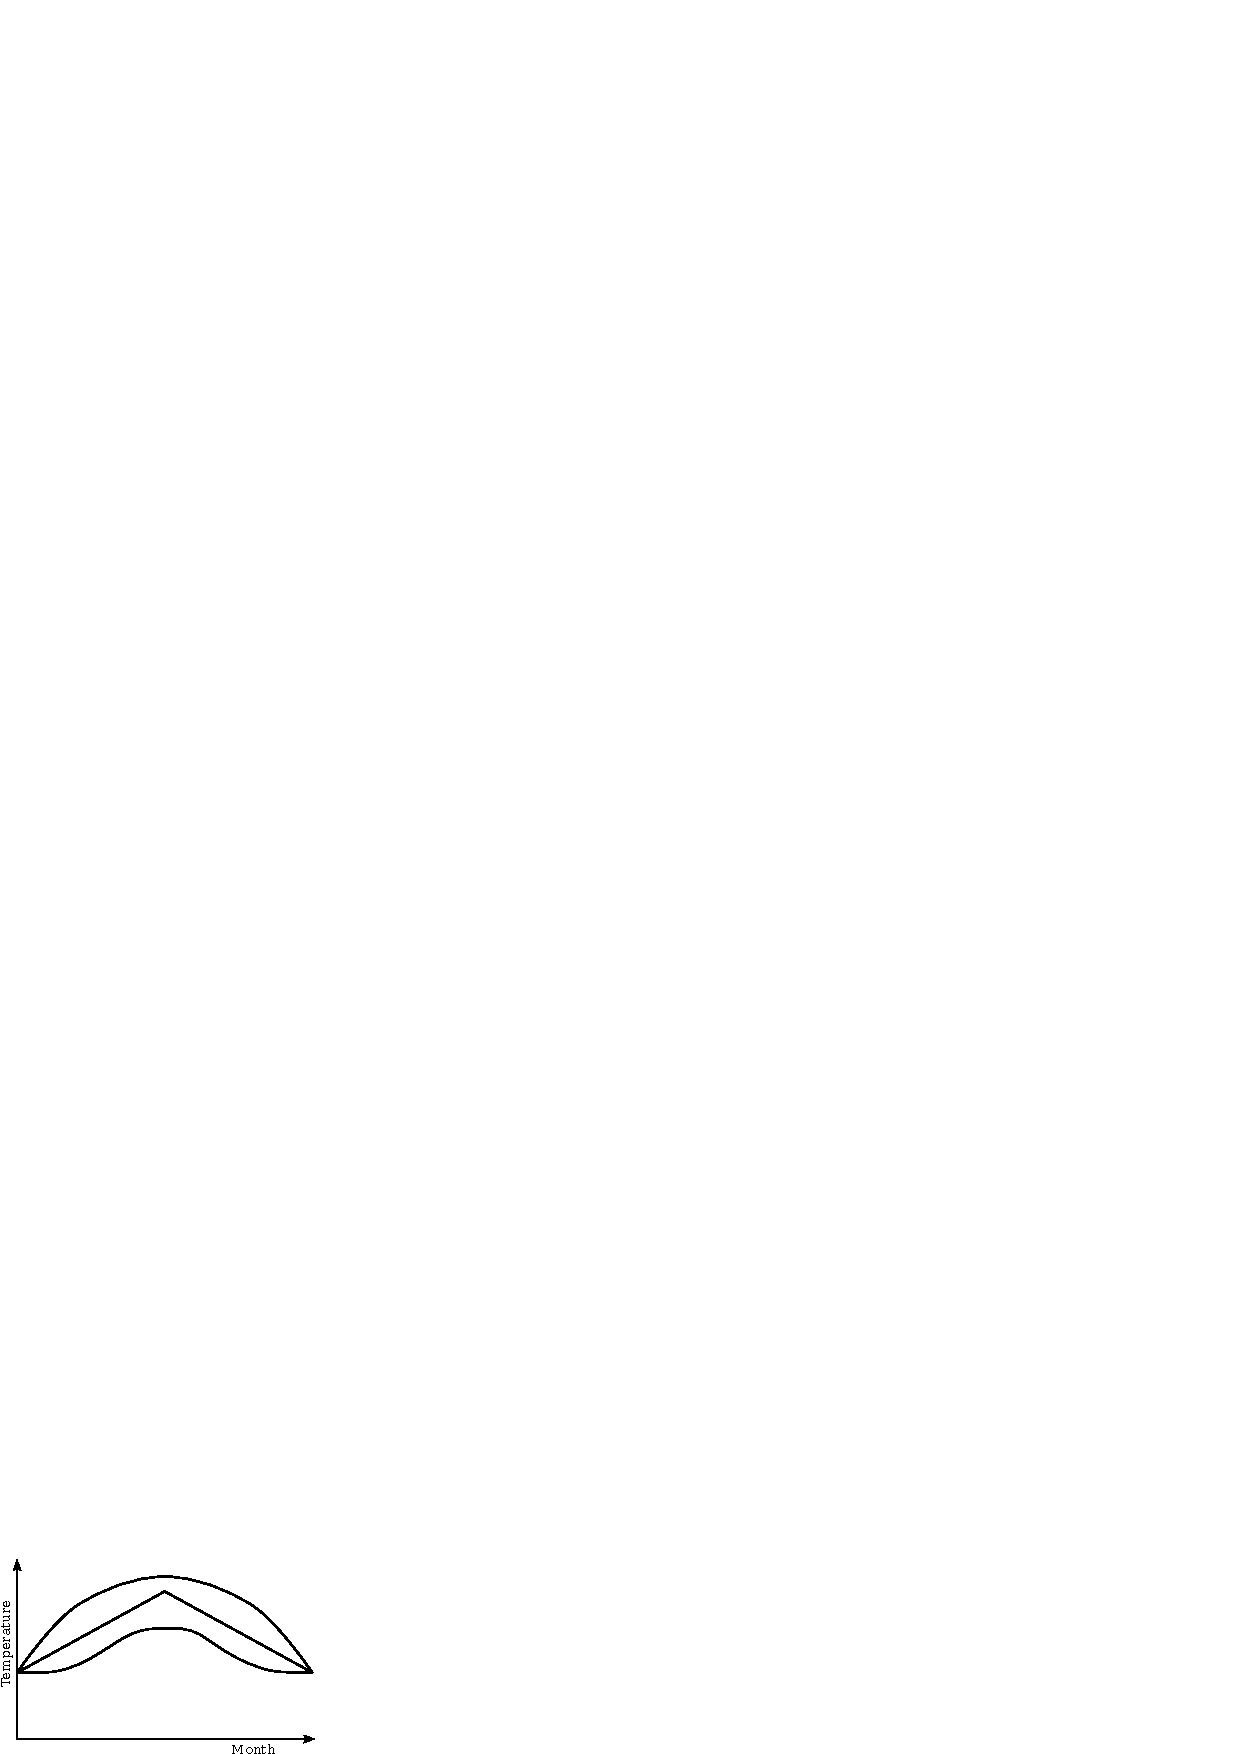
\includegraphics{graphics/temp.pdf}
\]

\item The number of gallons of milk you can buy with $\$5$ as the cost per gallon of
  milk increases

\[
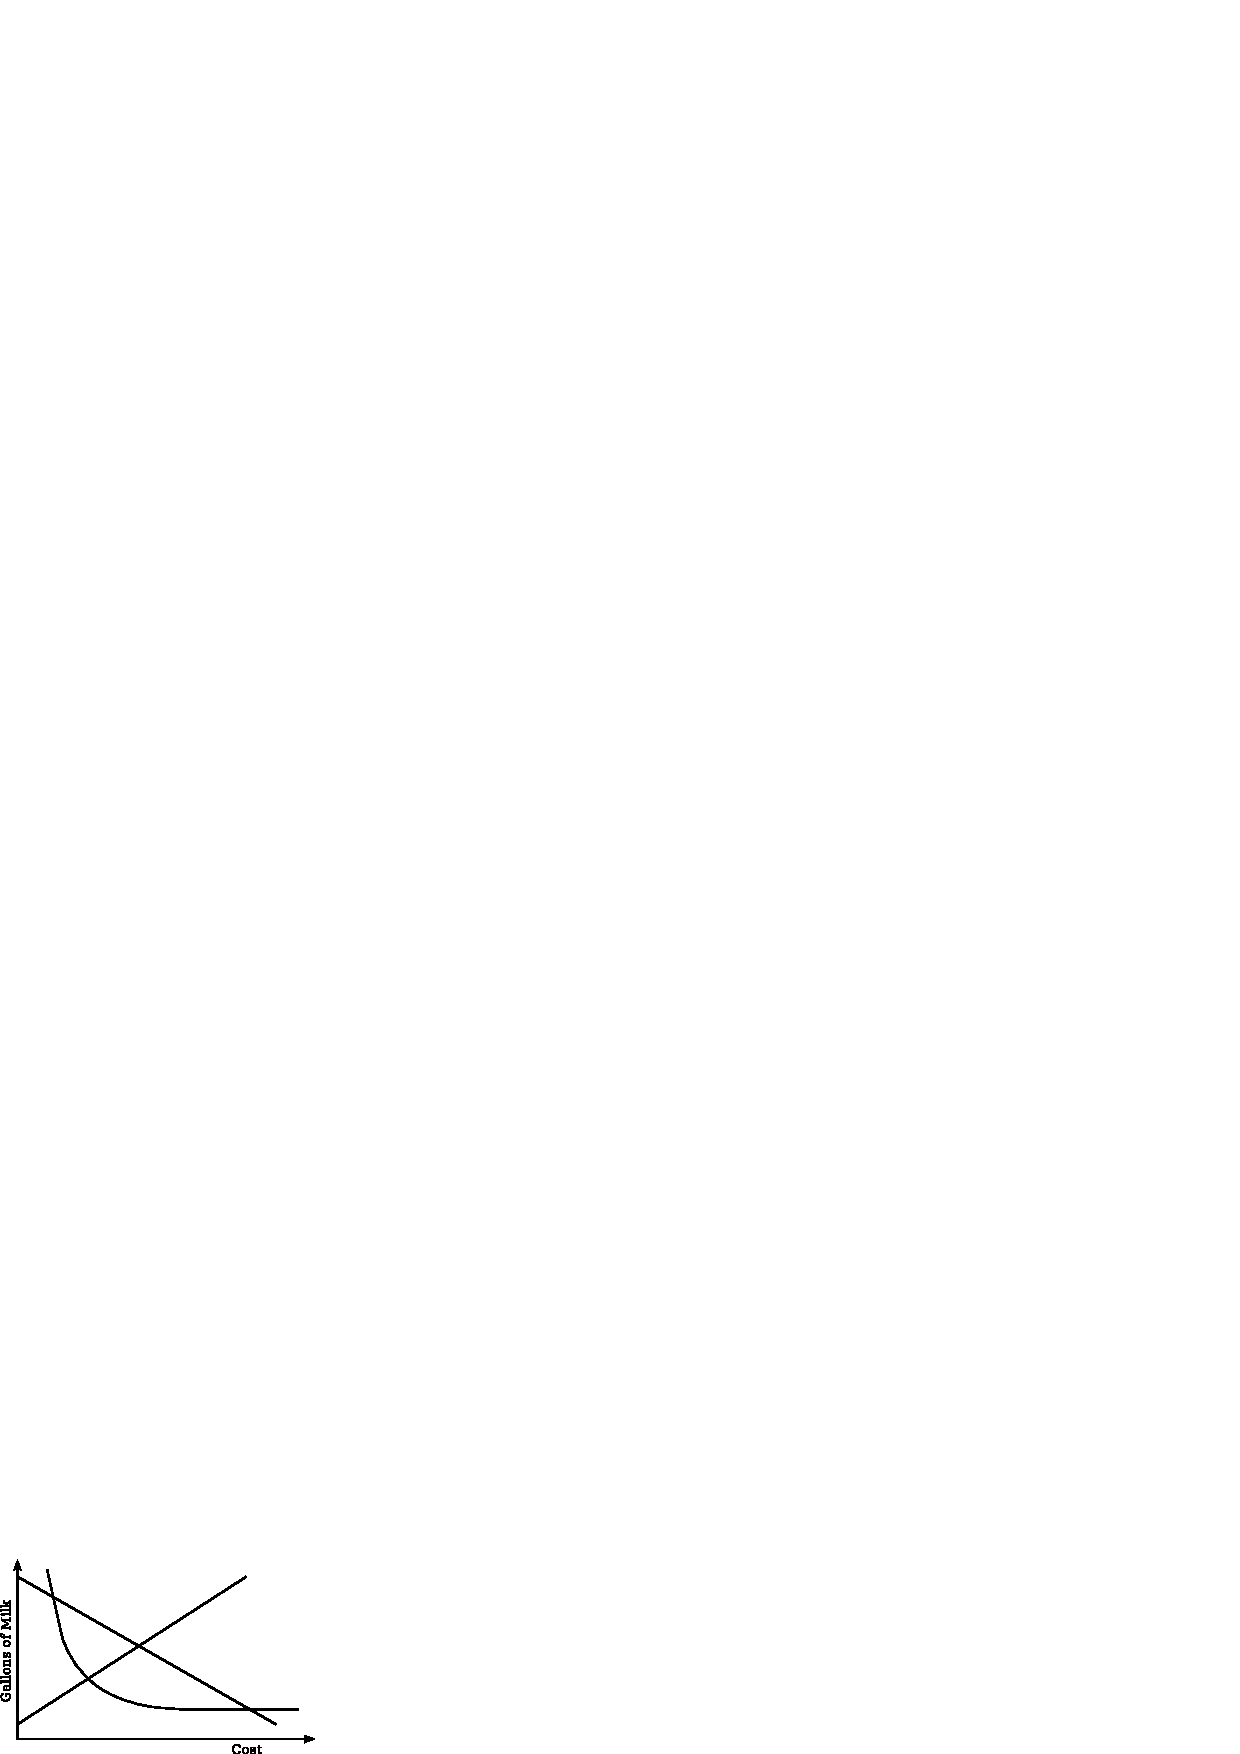
\includegraphics{graphics/milk.pdf}
\]

\end{enumerate}


\begin{instructorNotes}
\begin{enumerate}
    \item Part (a) is often controversial - make sure you take time to hear all students' opinions.
    \item All throughout, one key is paying attention to what each axis represents.  Some of them might be true if the vertical axis changed its meaning.
    \item On part (b), you might suggest that students try plugging in some numbers if they are stuck, or if they aren't convinced by the correct answer.  This problem again is frequently controversial.
\end{enumerate}
\end{instructorNotes}




\end{problem}



\begin{problem}
Water is poured at a constant rate into the three containers shown
below. Which graph corresponds to which container?

\begin{figure}[h]
\begin{center}
\includegraphics[scale=0.3]{graphics/2}
\end{center}
\end{figure}



\begin{instructorNotes}
\begin{enumerate}
    \item All of these problems bring out the idea that it's important not only to study if a quantity increases or decreases, but how it does those things.  Not all the world is linear! (Idea of concavity and calculus – studying when rates change – in general might be brought up here).
    \item Pay attention to the horizontal axis here and in the next problem - its meaning changes from problem to problem!
\end{enumerate}
\end{instructorNotes}
\end{problem}

\newpage

\begin{problem}
Water is poured at a constant rate into the six containers shown
below. Which graph corresponds to which container?

\begin{figure}[h]
\begin{center}
\includegraphics[scale=0.3]{graphics/3.pdf}
\end{center}
\end{figure}


\end{problem}



\end{document}

